\documentclass{beamer}
\usetheme{Singapore}
\usecolortheme{crane}
\usepackage{iwona}
\usepackage{graphicx}
\usepackage{amsmath}
\usepackage{mathdots}
\usepackage{amsthm}
\usepackage{amssymb}
\usepackage{hyperref}
\usepackage{lscape}
\usepackage{multicol}
\usenavigationsymbolstemplate{}
\def\insertnavigation#1{\relax}

\definecolor{mathorange}{HTML}{BC5E00}
\setbeamercolor{math text displayed}{fg=mathorange}

\title{Algebra, Calculus \& Probability Refresher}
\subtitle{MSc Week 0}
\author{Geraint Palmer\\Room: M/1.29\\\url{palmergi1@cardiff.ac.uk}\\}
\date{\tiny{Last updated \today}}

\begin{document}

\maketitle

\frame{
	\begin{block}{\begin{center}\huge{\textbf{\textit{Algebra}}}\end{center}}
  \vspace{5mm}
	\end{block}
}

\frame{
  \frametitle{Numbers}
  \begin{itemize}
    \item Integers: $$\mathbb{Z} = \{\dots, -3, -2, -1, 0, 1, 2, 3, \dots\}$$
    \item Rationals:
    $$\mathbb{Q} = \left\{ a \; | \; \exists \; p, q \in \mathbb{Z} \text{ for which } a = {p \over q}\right\}$$
    \item Real numbers: $$\mathbb{Z} \subset \mathbb{Q} \subset \mathbb{R}$$
  \end{itemize}
}

\frame{
  \frametitle{Exponents}
  For $a, b \in \mathbb{R^+}$, $x, y \in \mathbb{R}$:
  \vspace{5mm}
  \begin{multicols}{2}
    \begin{enumerate}
      \itemsep1.5em
      \item $a^x a^y = a^{x+y}$
      \item $a^0 = 1$
      \item $a^{-x} = {1 \over a^x}$
      \item $\left(a^x\right)^y = a^{xy}$
      \item $a^x b^x = (ab)^x$
      \item $a^{1 \over 2} = \sqrt{a}$
    \end{enumerate}
  \end{multicols}
}

\frame{
  \frametitle{Logarithms}
  $$\log_a{a^b} = b$$
  $$3^x = 81 \Leftrightarrow x = \log_3{81} = 4$$
}

\frame{
  \frametitle{Functions}
  Evaluate the function $f$ when $a = 4$, $b = 2$, $c = -5$:
  $$f(a, b, c) = {a \over b} + 4c - a^2c + 10\left(a + b\right)$$
  \pause
  Solution:
  \begin{align*}
    f(4, 2, -5)
      &= {4 \over 2} + \left(4 \times -5\right) - \left(4^2 \times -5\right) + 10\left(4 + 2\right)\\
      &= 2 - 20 - \left(16 \times -5\right) + 10\left(6\right)\\
      &= 2 - 20 + 80 + 60\\
      &= 122
  \end{align*}
}

\frame{
  \frametitle{Coordinates in the plane}
  Right handed Cartesian axes:
  \begin{center}
    $(1.3, 0.75)$\\
    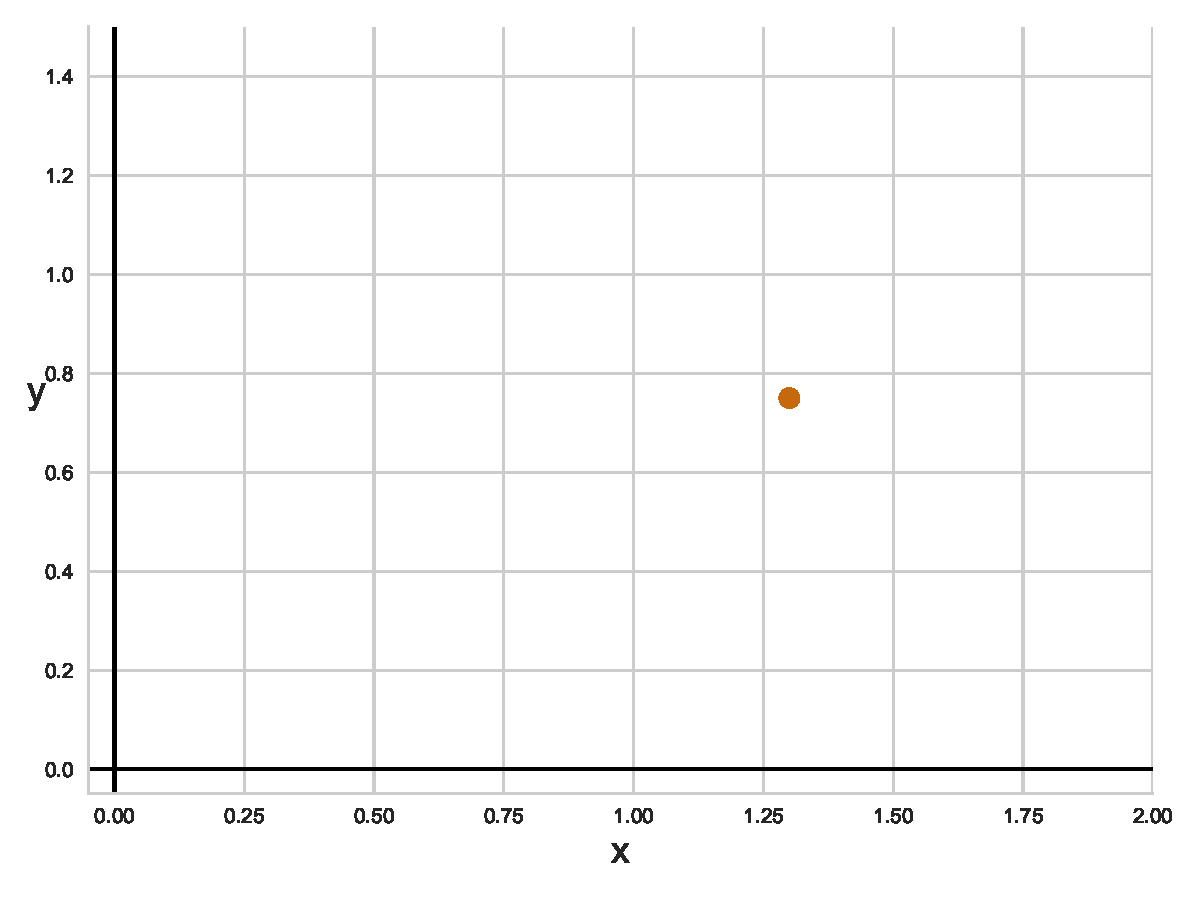
\includegraphics[width=7cm]{coordinate_system}\\
  \end{center}
  For $P = (x, y)$, $x/y$ is called the abscissa / ordinate of $P$.
}

\frame{
  \frametitle{Graphs}
  If $x$ and $y$ connected by an equation, then this relation can be represented
  by a curve or curves in the $(x, y)$ plane which is known as the graph of the
  equation.
  \begin{center}
    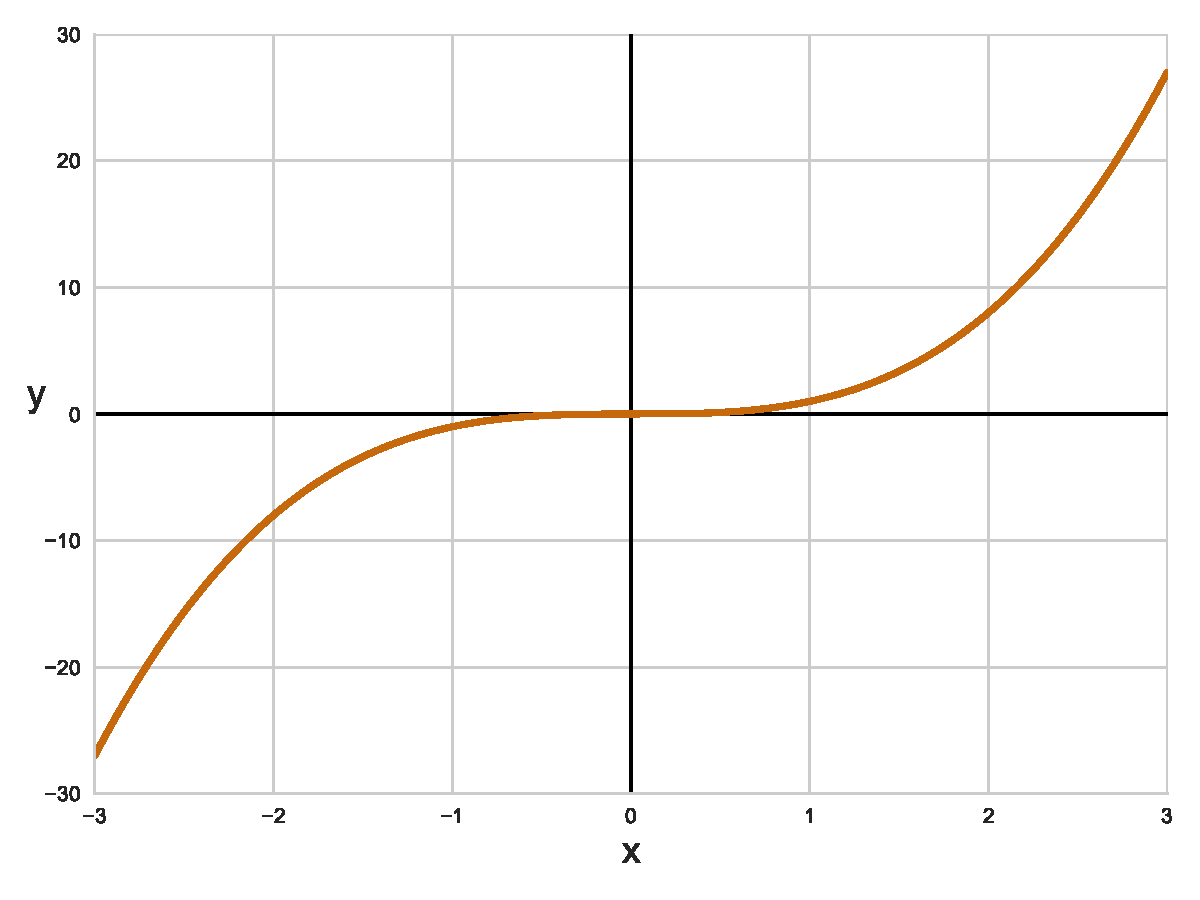
\includegraphics[width=7cm]{xcubed}
  \end{center}
  \begin{center}
  $y = x^3$
  \end{center}
}

\frame{
  \frametitle{Graphs}
  Graph of a straight line: $$y = mx + c$$
  \begin{itemize}
    \item $m$ is called the \emph{gradient} of the line.
    \item $c$ is called the $y$\emph{-intercept} of the line.
  \end{itemize}
}

\frame{
  \frametitle{Exercise}
  Find the equation for the line going through the points $\{(0.5, 3),(4, 1.1)\}$:
  \begin{center}
    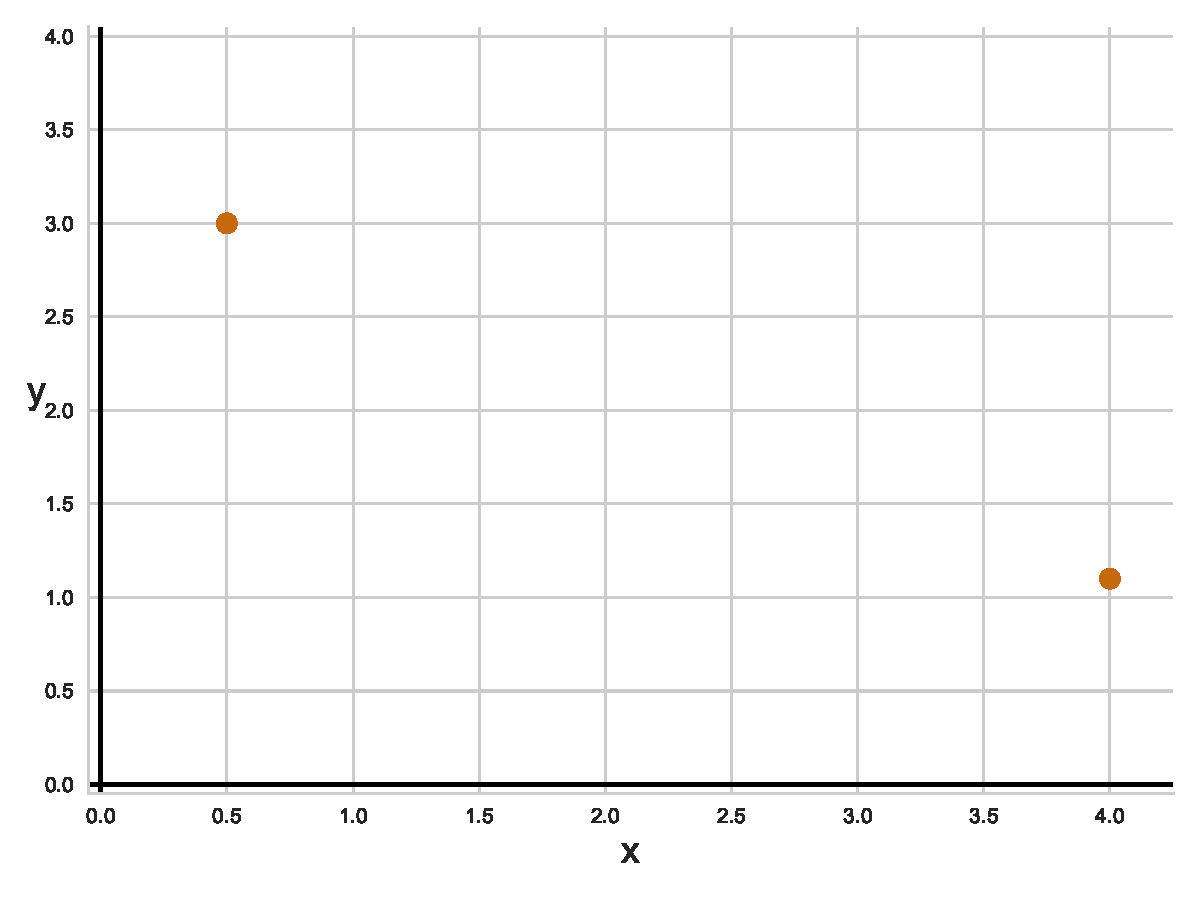
\includegraphics[width=7cm]{2points}
  \end{center}
}

\frame{
  \frametitle{Solution}
  General form of $y = mx + c$ through $\{(x_1, y_1),(x_2, y_2)\}$:
  $$\left.
    \begin{array}{@{}r@{\;}c@{\;}l@{}}
      y_1 & = & mx_1 + c\\
      y_2 & = & mx_2 + c
    \end{array}
  \right\}
  \Rightarrow m(x_1 - x_2) = y_1 - y_2$$
  which gives:
  $$\begin{array}{@{}r@{\;}c@{\;}l@{}}
    m & = & {y_1 - y_2 \over x_1 - x_2}\\[2mm]
    c & = & {x_2 y_1 - x_1 y_2 \over x_2 - x_1}
  \end{array}$$
}

\frame{
  \frametitle{Solution}
  So for $(x_1, y_1)=(0.5, 3)$ and $(x_2, y_2)=(4, 1.1)$ we have:
  $$\begin{array}{@{}r@{\;}c@{\;}l@{}}
    m & = & {1.9 \over -3.5} \approx -0.54\\[2mm]
    c & = & {11.45 \over 3.5} \approx 3.27
  \end{array}$$
  \begin{center}
    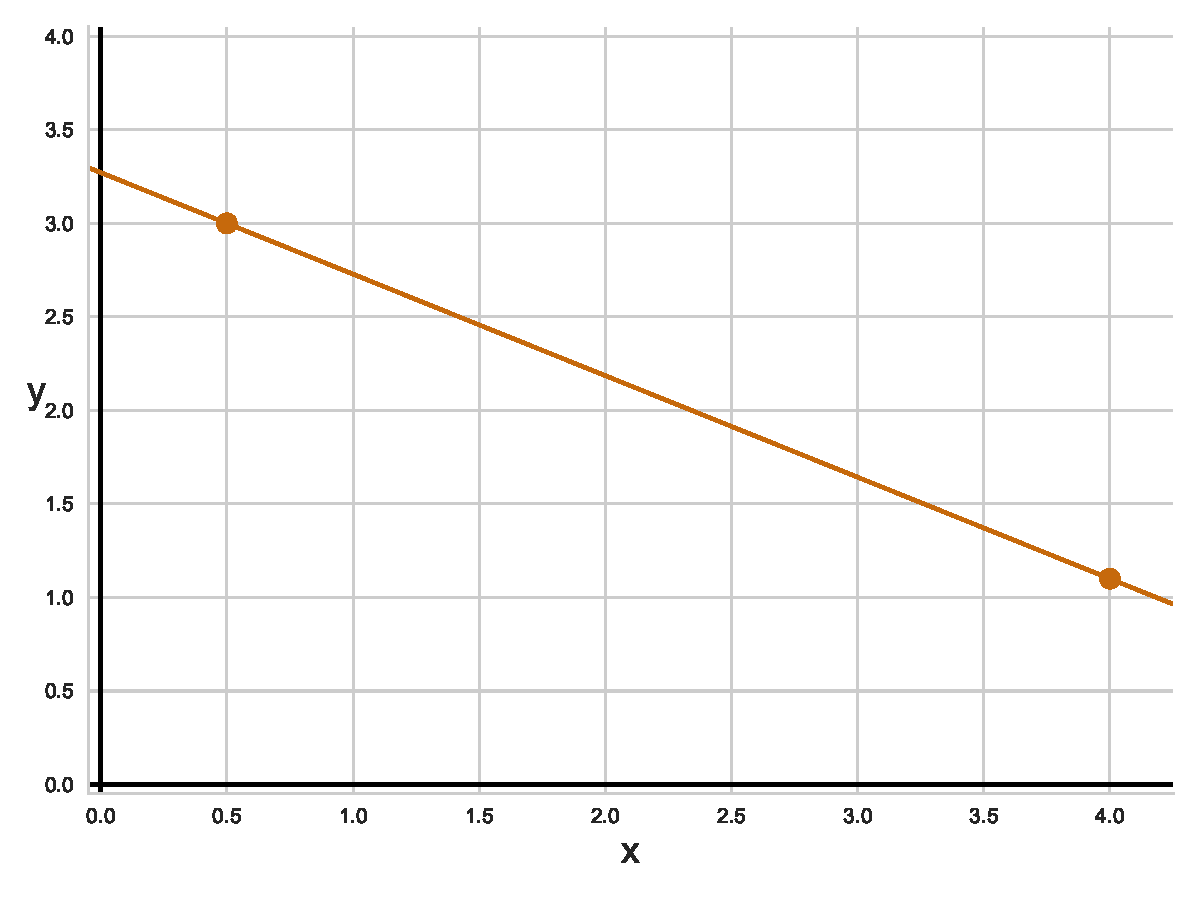
\includegraphics[width=7cm]{2pointsandline}
  \end{center}
}

\frame{
  \frametitle{Exercise}
  Where does the line $y = -0.54x + 3.27$ intersect the $y$-axis and the
  $x$-axis?\\
  \pause
  This is equivalent to solving:
  $$y = -0.54 \times 0 + 3.27$$
  and
  $$0 = -0.54x + 3.27$$
}

\frame{
  \frametitle{Solving Linear Equations}
  In linear equations are solved by multiplying or adding various constants.

  \begin{alignat*}{2}
    0 = -0.54x + 3.27 \quad
      &\Leftrightarrow
    0 - 3.27 &&= (-0.54x + 3.27) - 3.27\\
      &\Leftrightarrow
    -3.27 &&= -0.54x\\
      &\Leftrightarrow
    -3.27 \times {1 \over -0.54} &&= 0.54x \times {1 \over -0.54}\\
      &\Leftrightarrow
    6.06 &&\approx x
  \end{alignat*}
}

\frame{
  \frametitle{Quadratic}A ``quadratic'' is an expression of the form:
  $$ax^2 + bx + c$$
  \begin{itemize}
    \item $a$ is called the quadratic coefficient,
    \item $b$ is called the linear coefficient,
    \item $c$ is called the constant term or free term.
  \end{itemize}
}

\frame{
  \frametitle{Quadratic}
  \begin{center}
    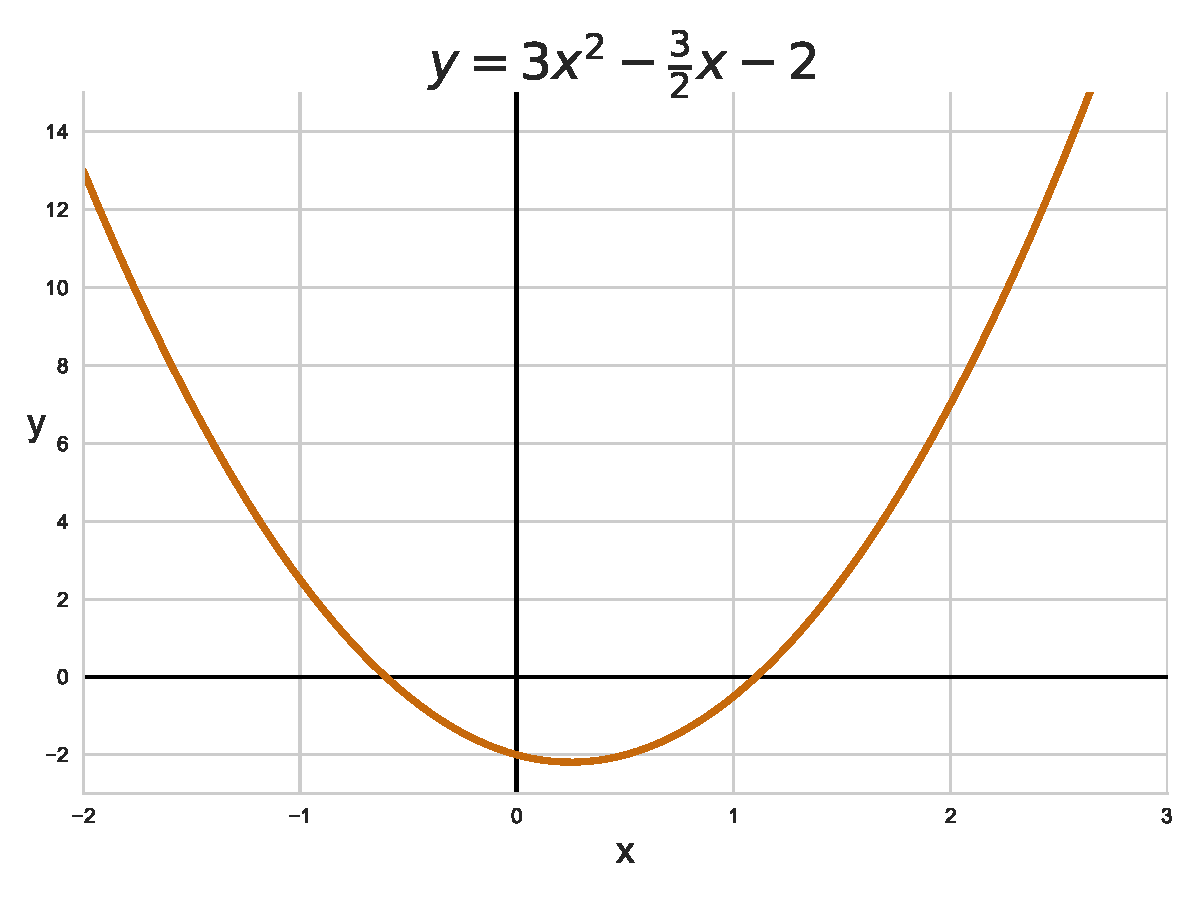
\includegraphics[width=7cm]{quadratic.png}
  \end{center}
}

\frame{
  \frametitle{Solving a Quadratic Equation}
  General solution of the equation:
  $$ax^2 + bx + c = 0$$
  is given by:
  $$x = {-b \pm \sqrt{b^2 - 4ac} \over 2a}$$
}

\frame{
  \frametitle{Exercise}
  Solve the equation:
  $$3x^2 - {3 \over 2} x - 2 = 0$$
}

\frame{
  \frametitle{Solution}
  From the previous formula we have:
  
  \begin{align*}
    x = {-b \pm \sqrt{b^2 - 4ac} \over 2a}
      &\Leftrightarrow
    x = {{3 \over 2} \pm \sqrt{\left({3 \over 2}\right)^2 - 4 \times 3 \times(-2)} \over 2 \times 3}\\
      &\Leftrightarrow
    x = {{3 \over 2} \pm \sqrt{{9 \over 4} + 24} \over 6}\\
      &\Leftrightarrow
    x = {3 \over 12} \pm {{1 \over 2} \sqrt{9 + 96} \over 6}\\
      &\Leftrightarrow
    x = {1 \over 4} \pm {\sqrt{105} \over 12}
  \end{align*}
}

\frame{
  \frametitle{Exercise}
  Solve the equation:
  $$4x^2 - 2x + 10 = 3$$
}

\frame{
  \frametitle{Solution}
  From the previous formula we have:

  \begin{align*}
    x = {-b \pm \sqrt{b^2 - 4ac} \over 2a}
      &\Leftrightarrow
    x = {2 \pm \sqrt{2^2 - 4 \times 4 \times 7} \over 2 \times 4}\\
      &\Leftrightarrow
    x = {2 \pm \sqrt{-108} \over 8}\\
      &\Leftrightarrow
    x = {2 \pm \sqrt{i^2108} \over 8}\\
      &\Leftrightarrow
    x = {2 \pm i\sqrt{3 \times 36} \over 8}\\
      &\Leftrightarrow
    x = {2 \pm 6i\sqrt{3}\over8} = {1 \over 4} \pm {3 \over 4} i\sqrt{3}
\end{align*}
}

\frame{
  \frametitle{Complex Numbers}
  $$i^2 = -1$$
  Complex numbers:
  $$\mathbb{C} = \left\{a + bi \; | \; a, b \in \mathbb{R} \right\}$$
  If $z = a + ib$:
  \begin{itemize}
    \item $a$ is the real part of $z$.
    \item $b$ is the imaginary part of $z$.
  \end{itemize}
}

\frame{
  \frametitle{Solving Systems of Equations}
  A system of equations is a collection of equations involving the same set of
  variables. For example:

  \begin{align*}
    3x + 2y &= 1\\
    2x - 2y &= -2
  \end{align*}
Various techniques can be used to solve such a problem.
}

\frame{
  \frametitle{Solution}
  First equation gives:
  $$3x + 2y = 1 \Rightarrow x = {1 - 2y \over 3}$$
  Substituting in to second equation gives:
  $$2\left(1 - 2y \over 3\right) - 2y = -2$$
  which implies:
  $$y = {4 \over 5}$$
  Substituting in to our expression for $x$ we get:
  $$x = -{1 \over5}$$
}

\frame{
  \frametitle{Shorthand notation}
  \begin{itemize}
    \item Summation: $$\sum_{i=1}^{n} a_i = a_1 + a_2 + a_3 + \dots + a_n$$
    \item Multiplication: $$\prod_{i=1}^{n} a_i = a_1 \times a_2 \times a_3 \times \dots \times a_n$$
  \end{itemize}
}

\frame{
  \frametitle{Examples}
  \begin{itemize}
    \item Summation:
    \begin{align*}
      \sum_{i=1}^4 i \times 2^{i}
        &= 1 \times 2 + 2 \times 2^2 + 3 \time 2^3 + 4\times 2^4\\
        &= 2 + 8 + 3 \times 8 + 4 \times 16 = 98
    \end{align*}
    \item Multiplication: $$\prod_{k=1}^3 k^{2} = 1 \times 2^2 \times 3^2 = 36$$
  \end{itemize}
}

\frame{
  \frametitle{Proof by Induction}
  Technique often used to prove algebraic relationships. Basic idea:
  \begin{itemize}
    \item Prove that something is true at the start.
    \item Prove that if something is true at point $k$ then it is true at point
    $k + 1$.
  \end{itemize}
  \only<1>{
    \begin{center}
      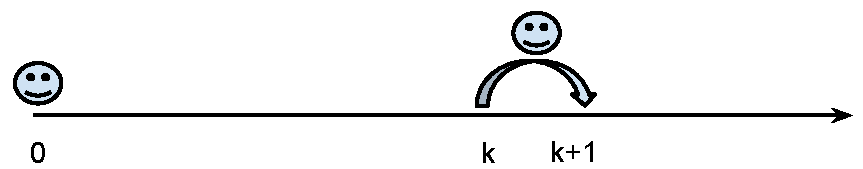
\includegraphics[width=7cm]{inductionpic}
    \end{center}
  }
  \only<2>{
    \begin{center}
      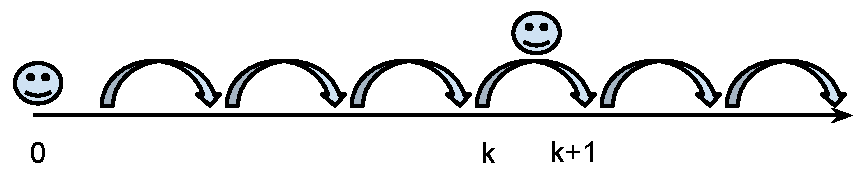
\includegraphics[width=7cm]{inductionpic1}
    \end{center}
  }
}

\frame{
  \frametitle{Exercise}
  Prove that: $$\sum_{i=0}^n i = {n(n + 1)\over 2}$$
}

\frame{
  \frametitle{Solution}
  \begin{itemize}
    \item True for $n = 0$?:
      $$\sum_{i=0}^0 i = 0 \; \text{ \color{black}{and} } \; {n(n + 1) \over 2} = 0$$
    \pause
    \item If true for $n=k$, true for $n=k+1$?:
      \begin{alignat*}{2}
        \sum_{i=0}^{k+1} i \; &= \; \sum_{i=0}^{k} i &&+ k + 1\\
        &= \; {k(k + 1) \over 2} &&+ k + 1\\
        &= \; {(k + 1)(k + 2) \over 2}
      \end{alignat*}
  \end{itemize}
}

\frame{
  \frametitle{Infinite Sums}
  \vfill
  $$\sum_{k=0}^\infty a^k = {a \over {1 - a}}$$
  \vfill
  $$\sum_{k=0}^\infty k a^k = {a \over {(1 - a)^2}}$$
  \vfill
  $$\sum_{k=0}^\infty {{a^k} \over k!} = e^a$$
  \vfill
  \small{\url{https://en.wikipedia.org/wiki/List_of_mathematical_series}}
}

\frame{
  \frametitle{Infinite Sums}
  \begin{align*}
  S &= \sum_{k=0}^\infty a^k\\
  S &= a^0 + a^1 + a^2 + a^3 + a^4 + \dots\\
  aS &= a^1 + a^2 + a^3 + a^4 + a^5 + \dots
  \end{align*}
  Consider $S - aS$:
  \begin{align*}
  S - aS &= a^0\\
  S - aS &= 1\\
  S(1 - a) &= 1\\
  S &= {1 \over (1-a)}
  \end{align*}
}

\frame{
  \begin{block}{\begin{center}\huge{\textbf{\textit{Calculus}}}\end{center}}
  \vspace{5mm}
  \end{block}
}

\frame{
  \frametitle{Functions}
  A function $f$ is a rule that assigns to each element $x$ in a set $D$ exactly
  one element, called $f(x)$, in a set $E$.
  \begin{center}
    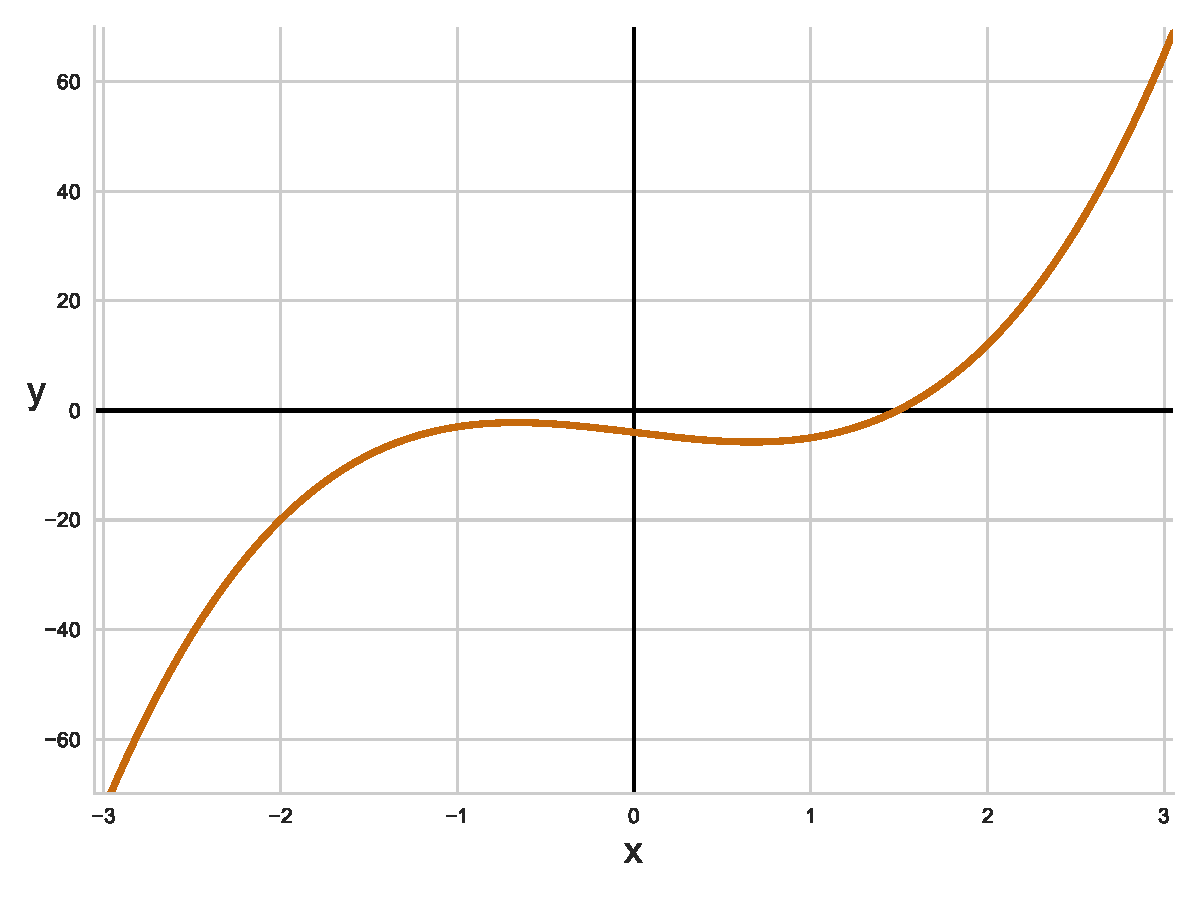
\includegraphics[width=7cm]{function}
  \end{center}
  \pause
  \begin{itemize}
    \item We usually consider functions for which the sets $D$ and $E$ are sets
    of real numbers.
    \item The set $D$ is called the domain of the function.
    \item The range of $f$ is the set of all possible values of $f(x)$ as $x$
    varies throughout the domain.
    \item A symbol that represents an arbitrary number in the domain of a
    function $f$ is call an independent variable.
    \item A symbol that represents a number in the range of $f$ is called a
    dependent variable.
  \end{itemize}
}

\frame{
  \frametitle{Example}
  \begin{center}
  $f(x) = 3x^3 - 4x - 4$
  \end{center}
  \begin{center}
    \includegraphics[width=7cm]{complicated_function}
  \end{center}
}

\frame{
  \frametitle{Tangent Curves}
  The tangent line to the curve $y = f(x)$ at the point $P = (a, f(a))$ is the line
  through $P$ with gradient:
  $$m = \lim_{x \to a}{f(x) - f(a) \over {x - a}}$$
}

\frame{
  \frametitle{Tangent Curves}
  \only<1>{
    \begin{center}
      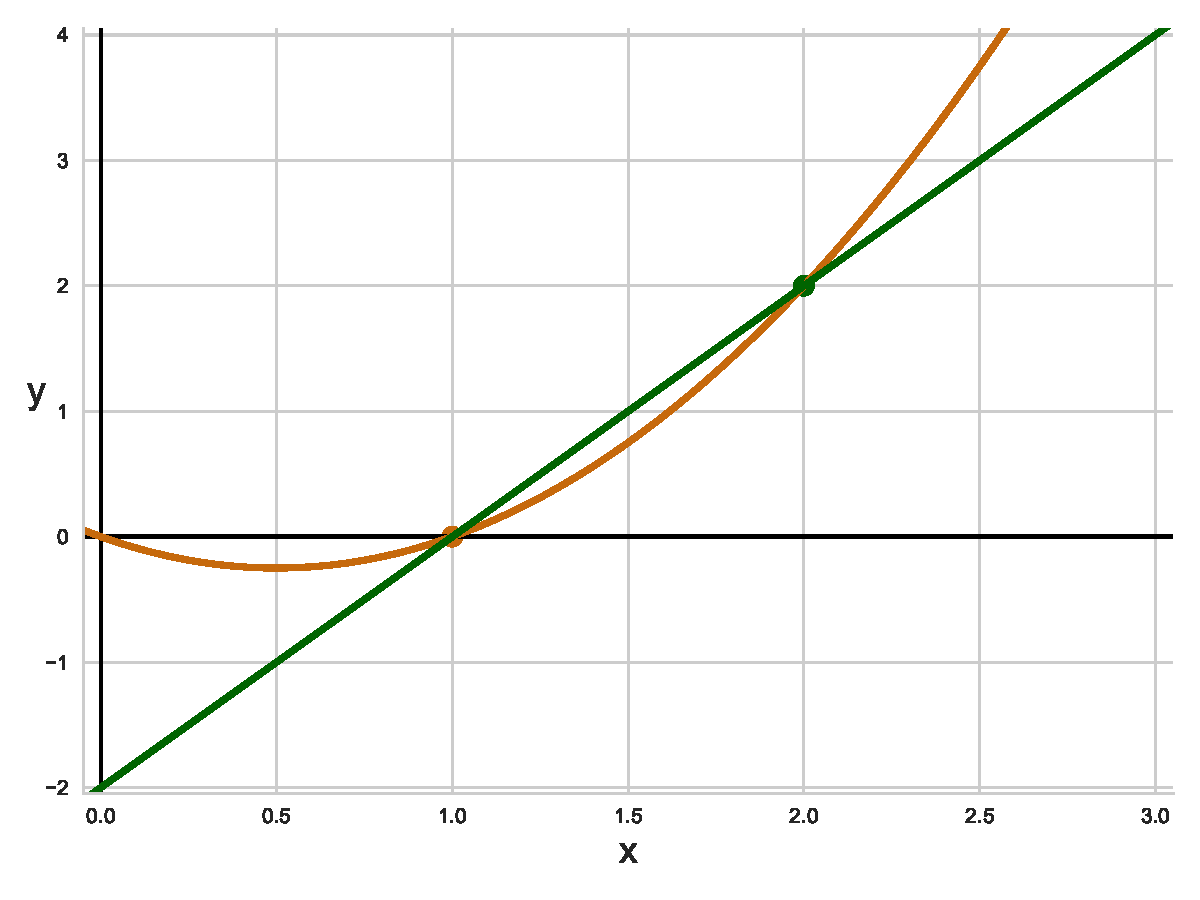
\includegraphics[width=7cm]{tangent_line}
    \end{center}
  }
  \only<2>{
    \begin{center}
      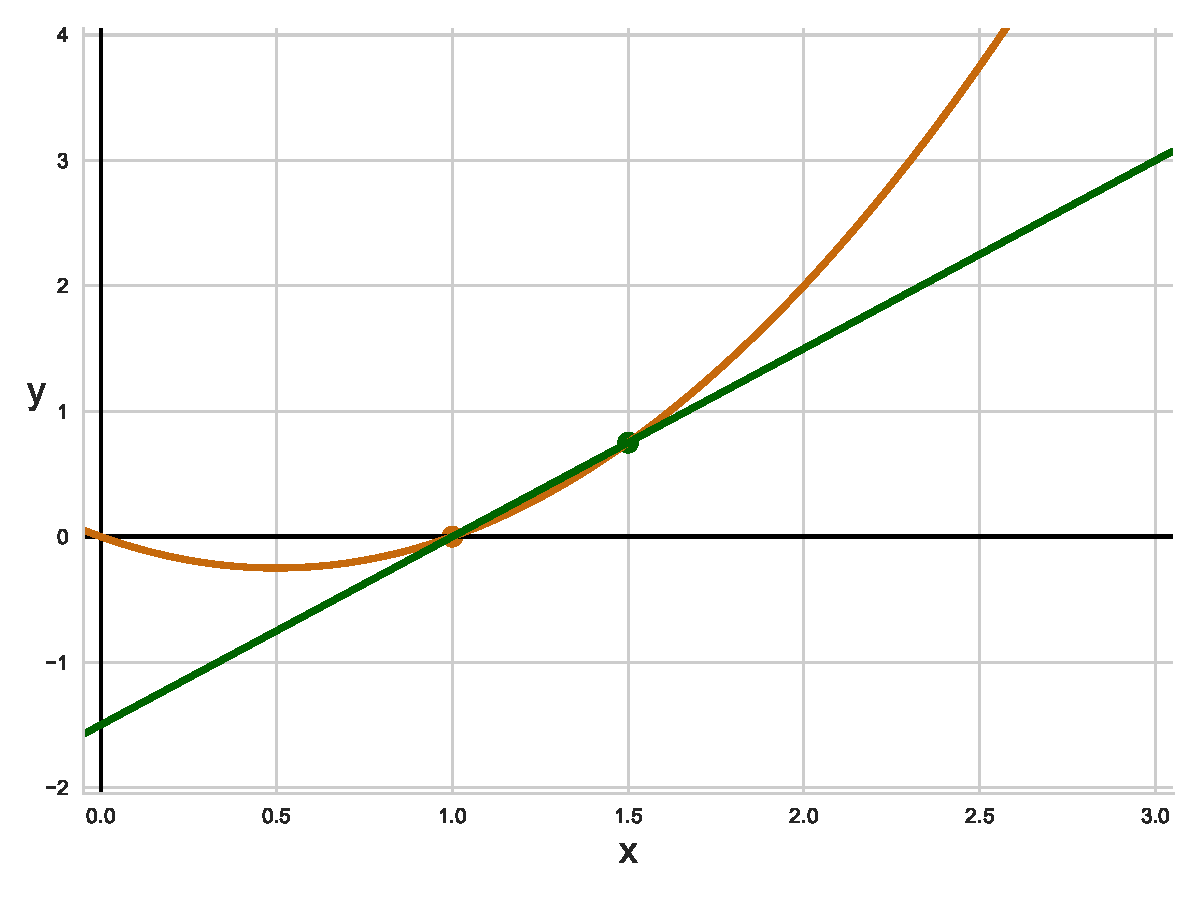
\includegraphics[width=7cm]{tangent_line_1}
    \end{center}
  }
  \only<3>{
    \begin{center}
      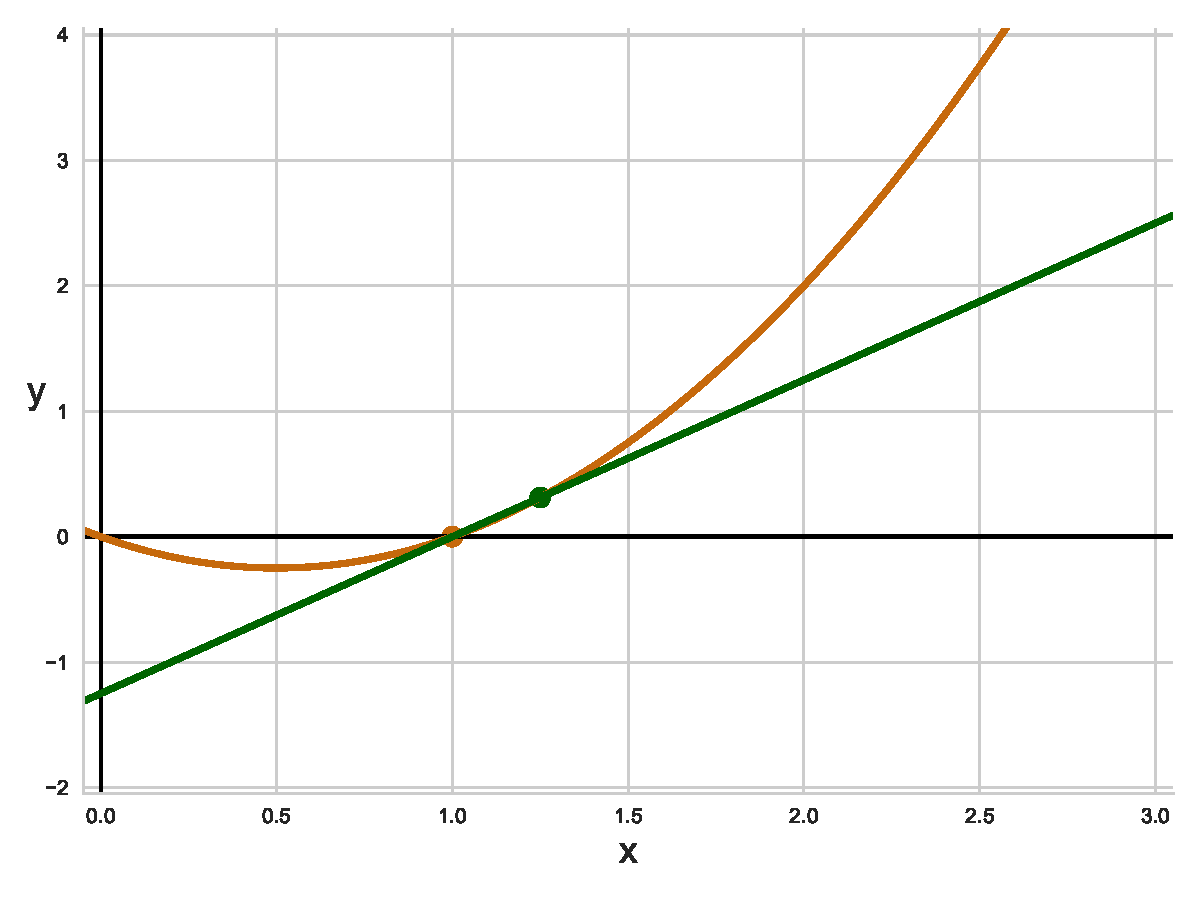
\includegraphics[width=7cm]{tangent_line_2}
    \end{center}
  }
  \only<4>{
    \begin{center}
      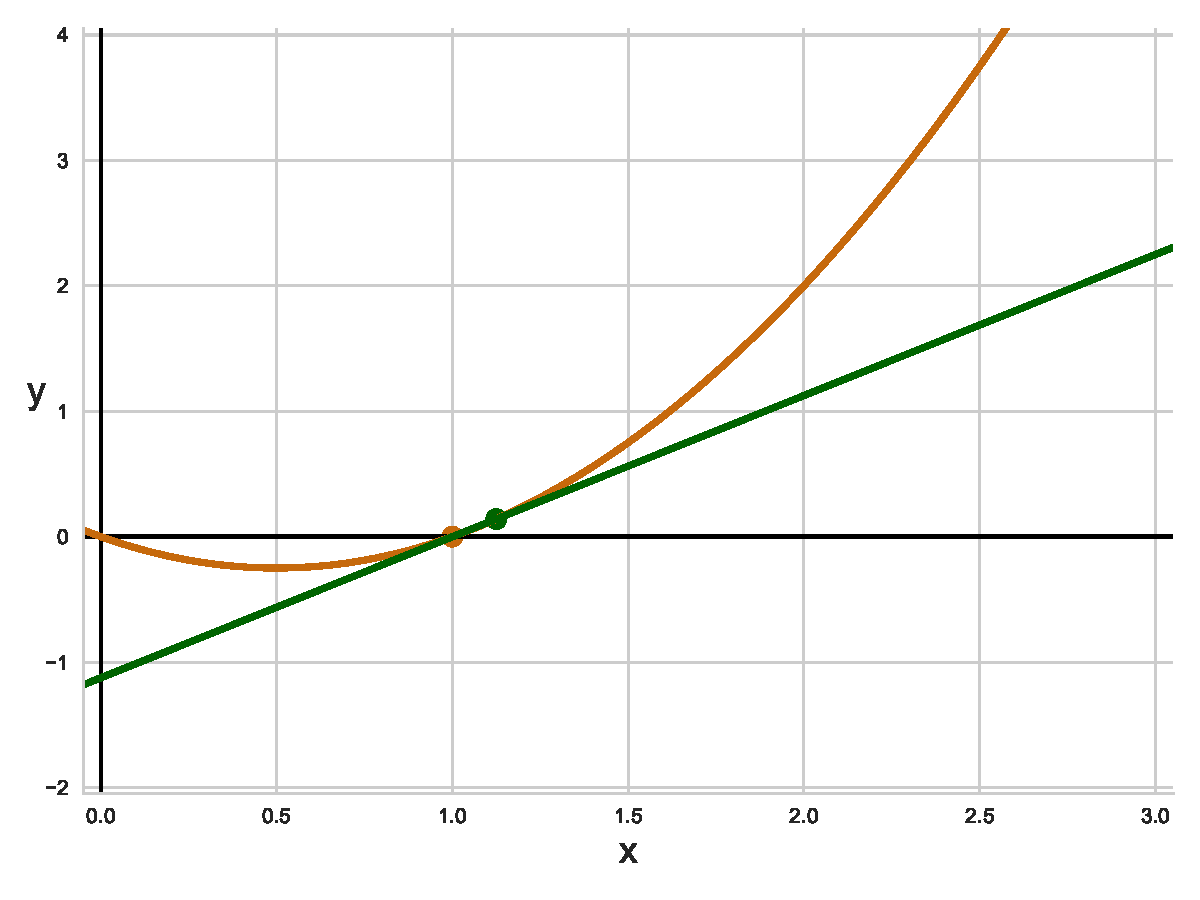
\includegraphics[width=7cm]{tangent_line_3}
    \end{center}
  }
  \only<5>{
    \begin{center}
      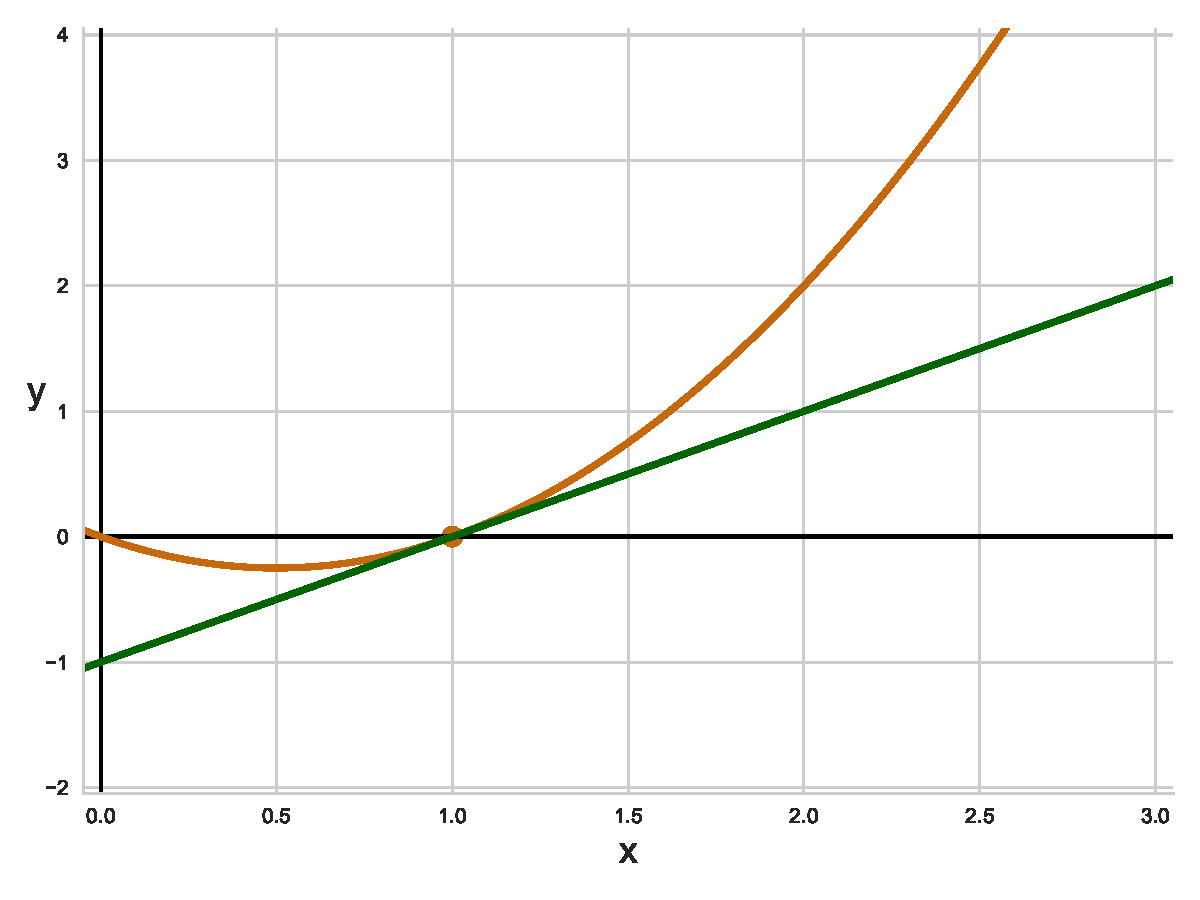
\includegraphics[width=7cm]{tangent_line_4}
    \end{center}
  }
}

\frame{
  \frametitle{Derivative}
    The derivative of a function $f$ at a number $a$, denoted by $f'(a)$ is:
    $$f'(a) = \lim_{h \to 0}{f(a + h) - f(a) \over h}$$
    \pause
    \\[20mm]
    For polynomials:
    \begin{align*}
      & f = x^n\\
      \implies & f' = nx^{n-1}
    \end{align*}
}

\frame{
  \frametitle{Exercise}
    Find the derivative of $$f(x) = x^2 - 3x + 2$$ at $x = 6$.
}

\frame{
  \frametitle{Solution}
  \begin{alignat*}{4}
    f(x) &= x^2 &&- 3x &&+ 2\\
    f(x) &= 1 \times x^2 &&- 3 \times x^1 &&+ 2 \times x^0\\
    & && &&&\\
    f'(x) &= 1 \times 2 \times x^{2 - 1} &&- 3 \times 1 \times x^{1 - 1} &&+ 2 \times 0 \times x^{0 - 1}\\
    f'(x) &= 2x^1 &&- 3x^0 &&+ 0\\
    f'(x) &= 2x &&- 3 &&\\
    & && &&\\
    f'(6) &= 2 \times 6 &&- 3 &&\\
    f'(6) &= 9 && &&
  \end{alignat*}
}

\frame{
  \frametitle{Rules of Differentiation}
  \begin{itemize}
    \item The Power Rule:
    $${d \over dx}\left(x^n\right) = nx^{n - 1}$$
    \item The Constant Multiple Rule:
    $${d \over dx}\left(cf(x)\right) = c{d \over dx}\left(f(x)\right)$$
    \item The Sum Rule:
    $$(f + g)' = f' + g'$$
\end{itemize}
}

\frame{
  \frametitle{Rules of Differentiation}
  \begin{itemize}
    \item The Product Rule:
    $$(fg)' = f'g + fg'$$
    \item The Quotient Rule:
    $$\left({f \over g}\right)' = {f'g - fg' \over g^2}$$
  \end{itemize}
}

\frame{
  \frametitle{The Chain Rule}
  If $f\left(g(x)\right) = f \circ g$:
  $$\left(f \circ g\right)' = \left(f' \circ g\right)g'$$
}

\frame{
  \frametitle{Exercise}
  Differentiate $F(x)=\sqrt{x^2 + 1}$.
}

\frame{
  \frametitle{Solution}
  If we let $f(x) = \sqrt{x} = x^{1 \over 2}$ and $g(x) = x^2 + 1$ then we have:
  $$f' = {1 \over 2}x^{-{1 \over 2}} = {1 \over 2\sqrt{x}}$$
  and
  $$g' = 2x$$
  Using the Chain Rule we have:
  \begin{align*}
    F'(x)
      &= \left({1 \over 2\sqrt{x^2 + 1}}\right)\left(2x\right)\\
      &= {x \over \sqrt{x^2 + 1}}
  \end{align*}
}

\frame{
  \frametitle{Table of Derivatives}
  $$\begin{array}{@{}l@{}}
    \displaystyle{{d \over dx}\sin(x) = \cos(x)}\\[3mm]
    \displaystyle{{d \over dx}\cos(x) = -\sin(x)}\\[3mm]
    \displaystyle{{d \over dx}\tan(x) = \sec^2(x)}\\[3mm]
  \end{array}$$
  \begin{center}
    \scriptsize{\url{http://www.math.wustl.edu/~freiwald/131derivativetable.pdf}}
  \end{center}
}

\frame{
  \frametitle{Natural Exponential Function}
  The mathematical constant $e$ can be defined as the real number such that:
  $${d \over dx}e^x = e^x$$
  \begin{center}
    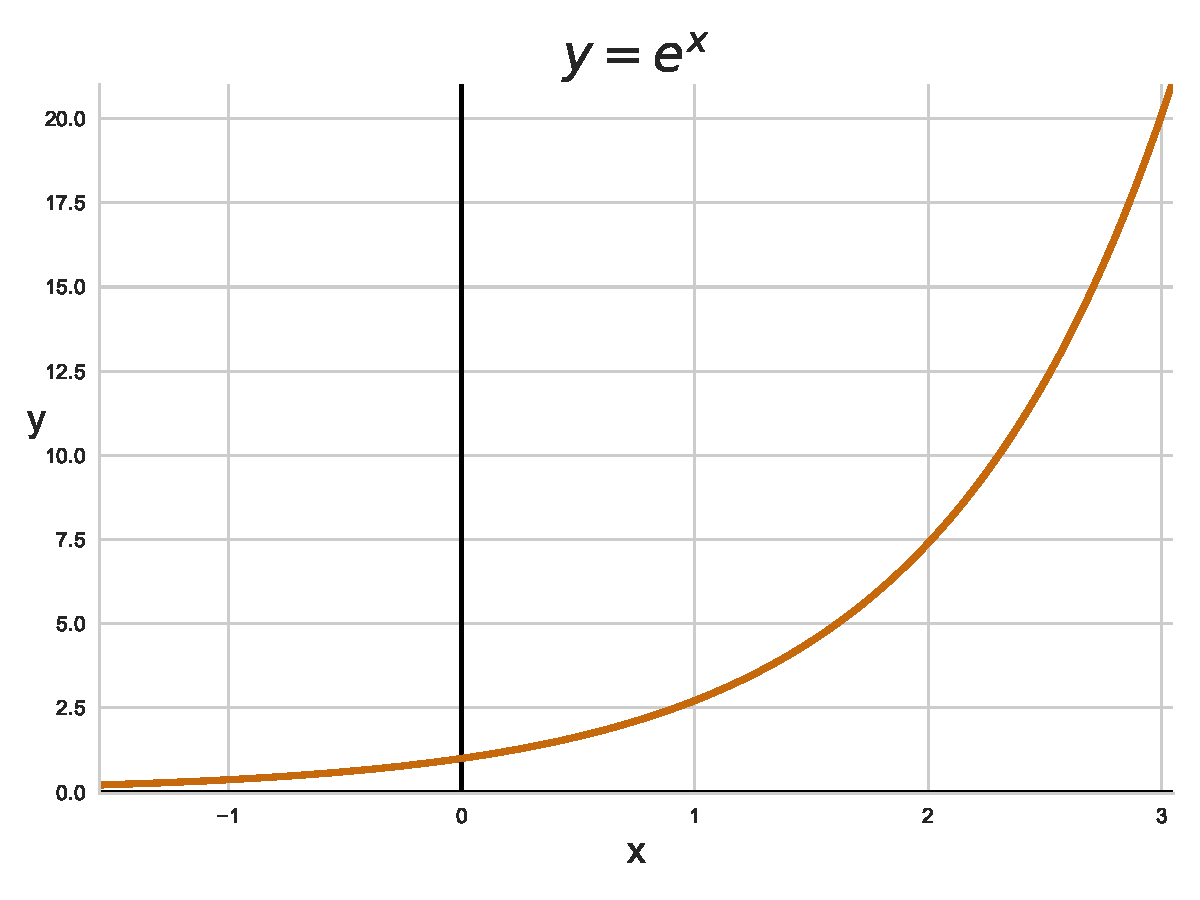
\includegraphics[width=7cm]{exp}
  \end{center}
}

\frame{
  \frametitle{Naural Logarithm}
  $$\ln x =\log_e x$$
  $$y = e^x \Leftrightarrow x = \ln y$$
}

\frame{
  \frametitle{Logarithms in Statistics}
  In the following graph the red dots are contracted by $\log$.
  This is a standard procedure sometimes used when analysing data.
  \begin{center}
    \includegraphics[width=7cm]{log_example}
  \end{center}
}

\frame{
  \frametitle{Area under a graph}
  \begin{center}
    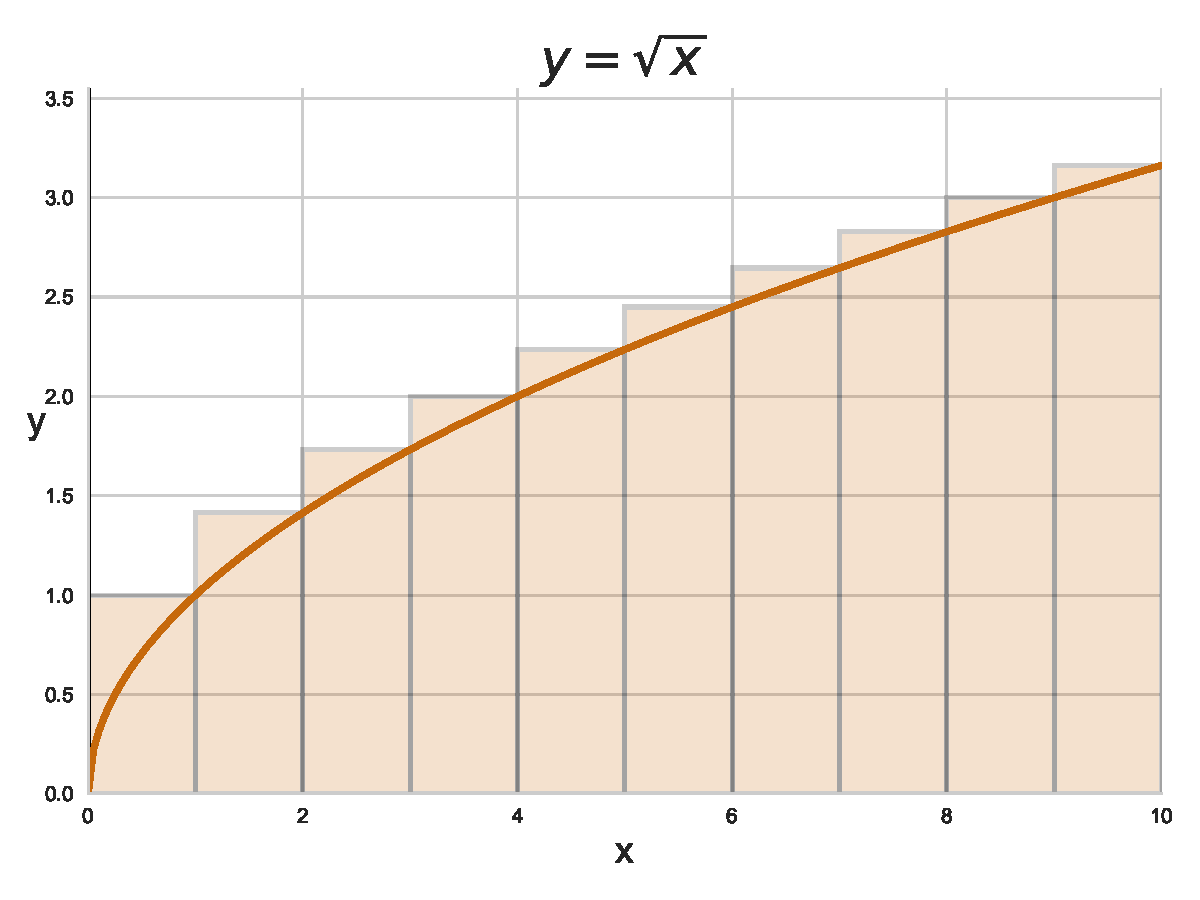
\includegraphics[width=7cm]{area_under_graph.pdf}
  \end{center}
}

\frame{
  \frametitle{Fundamental Theorem of Calculus}
  Let $f$, $F$ be continuous on $[a,b]$ then:\newline
  \begin{enumerate}
    \itemsep1.5em
    \item If $F(x) = \int_{a}^x f(t)dt$ then $F' = f$.
    \item $\int_{a}^b f(x)dx = F(b) - F(a)$
\end{enumerate}
\vspace{20mm}
\pause
$$\int f(x)dx = F(x) \; \text{ \color{black}{means} } \; {d \over dx}F=f$$
}

\frame{
  \frametitle{Tables of Indefinite Integrals}
  $$\begin{array}{@{}l@{}}
    \displaystyle{\int x^n dx = {x^{n + 1} \over n + 1} + C \qquad \qquad \color{black}{(n \ne -1)}}\\[3mm]
    \displaystyle{\int cf(x) dx = c \int f(x)dx}\\[3mm]
    \displaystyle{\int \left(f(x) + g(x)\right)dx = \int f(x)dx + \int g(x) dx}\\[3mm]
    \vdots
  \end{array}$$
  \begin{center}
    \scriptsize{\url{http://integral-table.com/downloads/single-page-integral-table.pdf}}
  \end{center}
}

\frame{
  \frametitle{Exercise}
  Calculate: $$\int{x^2 + \sin(x)dx}$$
  \vspace{20mm}
  \pause
  $$\int{x^2 + \sin(x)dx} = {x^3 \over 3} - \cos(x) + C$$
}

\frame{
  \frametitle{Integration by Parts}
    If $u = f(x)$ and $v = g(x)$: $$\int udv = uv - \int vdu$$
}

\frame{
  \frametitle{Exercise}
  Calculate: $$\int x\cos(x)dx$$
}

\frame{
  \frametitle{Solution}
  Letting $u = x$ and $dv = \cos(x)dx$ we have $du = dx$ and $v = \sin(x)$, thus:
  \begin{align*}
    \int x\cos (x)dx
      &= \int udv = uv - vdu\\
      &= x\sin(x) - \int \sin(x)dx\\
      &= x\sin(x) + \cos(x) + C
  \end{align*}
}

\frame{
  \frametitle{The Substitution Rule}
  If $u = g(x)$ then: $$\int f(g(x))g'(x)dx = \int f(u)du$$
}

\frame{
  \frametitle{Exercise}
  Calculate: $$\int x^3 \cos(x^4+2)dx$$
}

\frame{
  \frametitle{Solution}
  Letting $u = x^4 + 2$, we have $du =4x^3 dx$, thus:
  \begin{align*}
    \int x^3 \cos(x^4 + 2)dx
      &= \int \cos(u){1 \over 4}du\\
      &= {1 \over 4} \int \cos(u)du\\
      &= {1 \over 4}\sin(u) + C\\
      &= {1 \over 4}\sin(x^4 + 2)+C
  \end{align*}
}

\frame{
  \begin{block}{\begin{center}\huge{\textbf{\textit{Probability}}}\end{center}}
  \vspace{5mm}
  \end{block}
}

\frame{
  \frametitle{Random Variables}
  In trials where the outcome is numerical, the outcomes are values of random
  variables.\\
  \vspace{0.5cm}
  Example: A coin is spun 3 times, how many heads appear?
  Denote the random variable associated with the number of heads by $X$.
  Denote the sample space by $S_X$ then:
  $$S_X = \{0, 1, 2, 3\}$$
}

\frame{
  \frametitle{Discrete Probability Distributions}
  For a probability distribution $P(X = x_i) = p_i$:\\
  \begin{itemize}
    \itemsep1.5em
    \item $0 \leq p_i \leq 1$
    \item All probabilities sum to $1$:
    \begin{itemize}
      \itemsep1.5em
      \item $\sum_{i=1}^n p_i = 1$ if $X$ has $n$ possible outcomes
      \item $\sum_{i=1}^\infty p_i = 1$ if $X$ has a countably infinite set of outcomes
    \end{itemize}
  \end{itemize}
}

\frame{
  \frametitle{Exercise}
  Write down the state space and probability distribution for the random
  variable $X$ associated with the rolling of a six sided die.
  \pause
  $$S_X = \{1, 2, 3, 4, 5, 6\}$$
  \begin{center}
    \begin{tabular}{r|cccccc}
      $x_i$ & 1 & 2 & 3 & 4 & 5 & 6 \\
      \hline
      \\[-1em]
      $P(X=x_i)$ & ${1 \over 6}$ & ${1 \over 6}$ & ${1 \over 6}$ & ${1 \over 6}$ & ${1 \over 6}$ & ${1 \over 6}$
    \end{tabular}
  \end{center}
}

\frame{
  \frametitle{Cumulative Distribution for Discrete Random Variables}
  For $P(X=x_i) = p_i$ the cumulative distribution $F(x) = P(X \leq x)$:
  $$F(x) = \sum_{i=1}^{x}P(X = x_i)$$
}

\frame{
  \frametitle{Exercise}
  Write down the cumulative probability distribution for the random variable
  $X$ associated with the rolling of a six sided dice.
  \pause
  \begin{center}
    \begin{tabular}{r|cccccc}
      $x_i$ & 1 & 2 & 3 & 4 & 5 & 6 \\
      \hline
      \\[-1em]
      $P(X = x_i)$ & ${1 \over 6}$ & ${1 \over 6}$ & ${1 \over 6}$ & ${1 \over 6}$ & ${1 \over 6}$ & ${1 \over 6}$\\[2mm]
      \hline
      \\[-1em]
      $F(x_i)$ & ${1 \over 6}$ & ${2 \over 6}$ & ${3 \over 6}$ & ${4 \over 6}$ & ${5 \over 6}$ & $1$\\[2mm]
    \end{tabular}
  \end{center}
}

\frame{
  \frametitle{Mean and Variance}
  Mean / Average / Expected Value:
  $$E(X) = \sum_{i=1}^n x_i p_i$$
  Variance:
  $$Var(X) = \sum_{i=1}^n \left(x_i - E(X)\right)^2 p_i$$
}

\frame{
  \frametitle{Exercise}
  Calculate the mean and variance for the random variable $X$ associated with
  the rolling of a six sided dice.\\
  \pause
  \vspace{5mm}
  Mean:
  \begin{align*}
    E(X) &= {0 \over 6} + {1 \over 6} + {2 \over 6} + {3 \over 6} + {4 \over 6} + {5 \over 6} + {6 \over 6}\\
    &= 3.5
  \end{align*}
  Variance:
  \small{
  \begin{align*}
    Var(X) &= {(0 - 3.5)^2 \over 6} + {(1 - 3.5)^2 \over 6} + {(2 - 3.5)^2 \over 6} + {(3 - 3.5)^2 \over 6}\\
    &+ {(4 - 3.5)^2 \over 6} + {(5 - 3.5)^2 \over 6} + {(6 - 3.5)^2 \over 6}\\
    &\approx 2.9
  \end{align*}
  }
}

\frame{
  \frametitle{Continuous Random Variables}
  The random variable $X$ is the time from $t = 0$ until a light bulb fails.
  $X$ is a continuous random variable, defined for the continuous variable
  $t \geq 0$, and is not a countable list of values.\\
  \vspace{5mm}
  Define a probability density function $f(x)$ over $\mathbb{R}$:
  \begin{itemize}
    \item $f(x) \geq 0$
    \item $\int_{-\infty}^{\infty}f(x)dx = 1$
    \item for any $x_1 < x_2$: $$P(x_1 \leq X \leq x_2) = \int_{x_1}^{x_2} f(x)dx$$
  \end{itemize}
}

\frame{
  \frametitle{Continuous CDF}
  $$F(x) = P(X \leq x) = \int_{-\infty}^x f(u)du$$
}

\frame{
  \frametitle{Mean and Variance of Continuous Random Variables}
  Mean: $$E(X) = \int_{-\infty}^{\infty}x f(x)dx$$
  Variance: $$Var(X) = \int_{-\infty}^{\infty} \left(x - E(X)\right)^2 f(x)dx$$
}

\frame{
  \frametitle{Exercise}
  Find the mean of the negative exponential distribution:
  $$f(x) = \lambda  e^{-\lambda x} \text{ \color{black}{defined for} } 0 < x < \infty$$
}

\frame{
  \frametitle{Solution}
  \begin{alignat*}{2}
  E(X) &= \int_0^\infty x f(x) dx\\
  &= \lambda \int_0^\infty x e^{-\lambda x} dx\\
  &= \lambda \left(uv - \int v du \right)_0^\infty\\
  &= \lambda \left[{x \over \lambda} e^{-\lambda x} + \int {1 \over \lambda} e^{-\lambda x} \right]_0^\infty\\
  &= \lambda \left[{x \over \lambda} e^{-\lambda x} + {1 \over \lambda^2} e^{-\lambda x} \right]_0^\infty\\
  &= \left[xe^{-\lambda x} + {1 \over \lambda} e^{-\lambda x} \right]_0^\infty\\
  &= 0 - 0 - 0 + {1 \over \lambda} = {1 \over \lambda}
  \end{alignat*}
}

\frame{
  \frametitle{Support Material}
  \begin{center}
    \url{https://intranet.cardiff.ac.uk/students/your-study/study-skills/maths-support}
    \url{https://github.com/drvinceknight/MSc_week_0/wiki}
  \end{center}
}

\end{document}
